\documentclass[twoside,colorback,accentcolor=tud4c,11pt]{tudreport}
%\usepackage{ngerman}
\usepackage{german} %damit euro zeichen richtig
\usepackage{eurosym}
\usepackage[stable]{footmisc}
\usepackage[ngerman,pdfview=FitH,pdfstartview=FitV]{hyperref}
\usepackage{array}
\usepackage{booktabs}
\usepackage{multirow}
\usepackage{longtable}
\newcolumntype{L}[1]{>{\raggedright\let\newline\\\arraybackslash\hspace{0pt}}m{#1}}
\usepackage{listings}
\lstdefinestyle{BashInputStyle}{
	language=bash,
    basicstyle=\ttfamily,
	%numbers=left,
	%	numberstyle=\tiny,
	%	numbersep=3pt,
	frame=tb,
	frameshape={RYR}{Y}{Y}{RYR},
	columns=fullflexible,
	backgroundcolor=\color{gray!20},
	linewidth=0.95\linewidth,
	xleftmargin=0.1\linewidth,
  showspaces=false,
showtabs=false,
breaklines=true,
showstringspaces=false,
breakatwhitespace=true,
belowskip=1.2em,
aboveskip=1.2em,
} 

%defining a blue link:
\newcommand{\mylink}[2] {	\href{#1}{	\textit{\textcolor{blue}{#2}}}}


\newlength{\longtablewidth}
\setlength{\longtablewidth}{0.675\linewidth}

\title{Project Ballbot}
\subtitle{Markus Lamprecht \\ Florian M\"uller \\ Michael Suffel}
%\subsubtitle{email: \textaccent{tud-design@pro-kevin.de}}
%\uppertitleback{(\textaccent{\textbackslash uppertitleback})}
%\lowertitleback{(\textaccent{\textbackslash lowertitleback})\hfill\today}
\institution{TU Darmstadt, RTM}

\begin{document}
\maketitle
\tableofcontents


\chapter{Item - List}
\begin{tabular}{l l l l l}
	Item & \# & W.[g] & Weblink & Picture\\
	OpenCR Board (Controlling the motors, IMU)&1&60&\mylink{https://github.com/ROBOTIS-GIT/OpenCR/wiki/Hardware_Specification\#specification}{github\_wiki} 
	&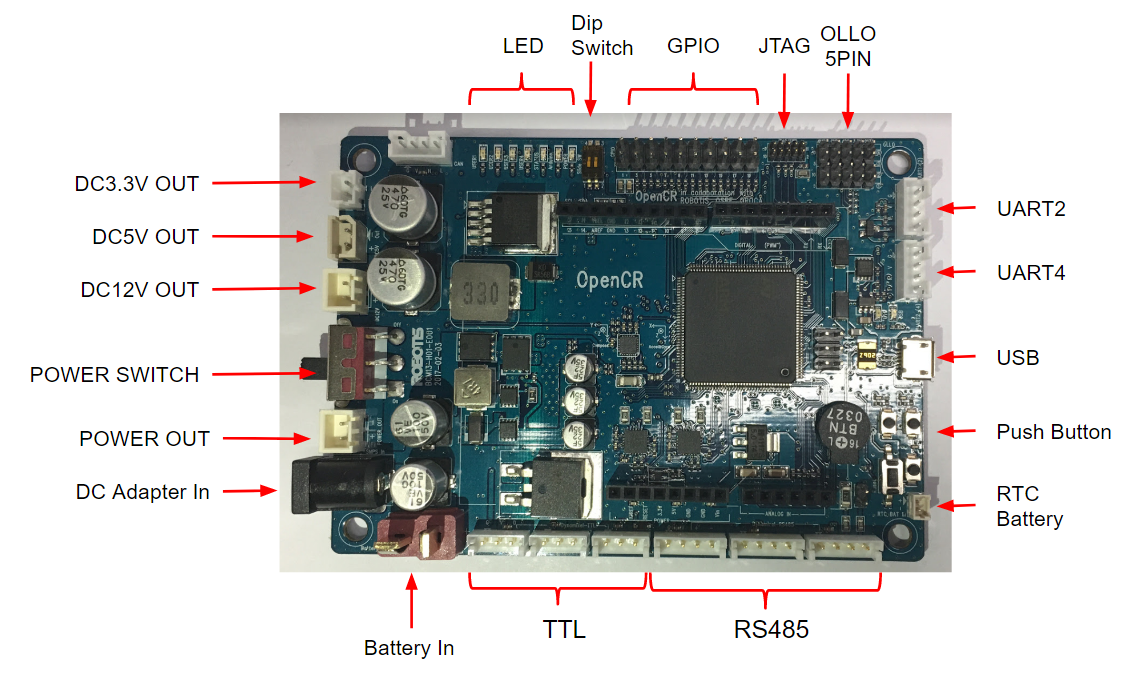
\includegraphics[width=0.1\textwidth]{img/opencr.png}  \\
	
	
	UpBoard (Main PC)&1 &96 & \mylink{https://up-shop.org/up-boards/44-up-board-4gb-ram-64-gb-emmc.html}{\EUR{127}}
	&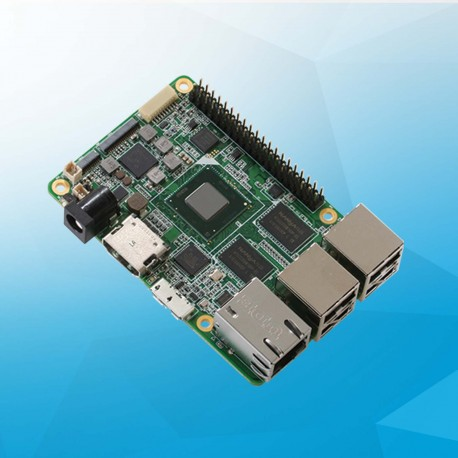
\includegraphics[width=0.1\textwidth]{img/upboard.jpg} \\
	
	Intel RealSense R200&1& 9.4& \mylink{https://www.intel.de/content/www/de/de/support/articles/000023534/emerging-technologies/intel-realsense-technology.html}{datasheet, \EUR{84.15}}&
	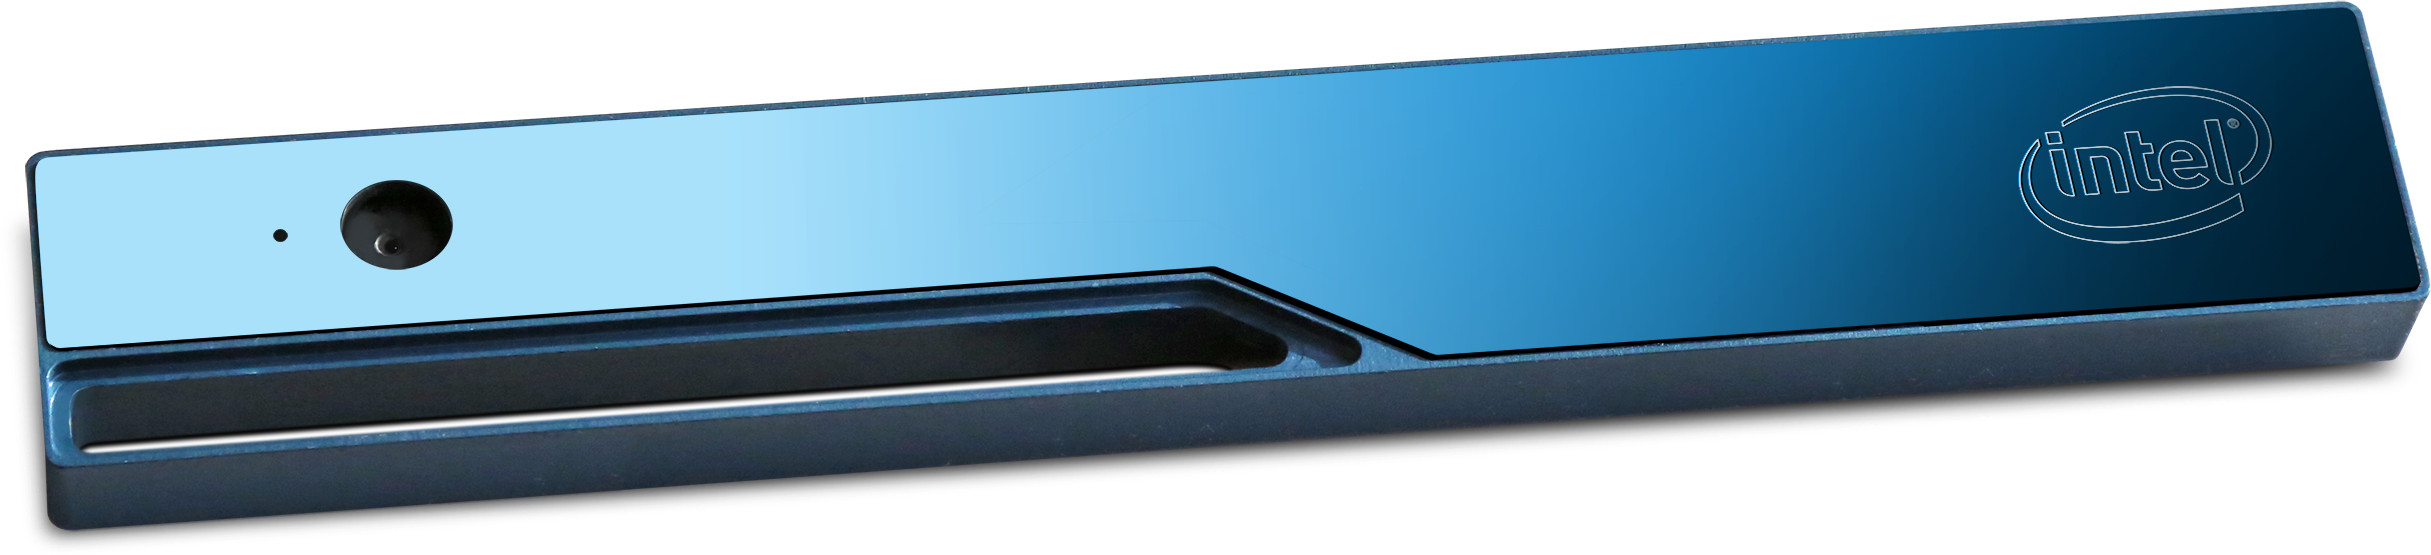
\includegraphics[width=0.1\textwidth]{img/r200.jpg} \\
	
	Laser Distance Sensor&1 &124 &\mylink{https://wiki.ros.org/hls_lfcd_lds_driver?action=AttachFile\&do=view\&target=LDS_Basic_Specification.pdf}{specs, \EUR{100}} & 
	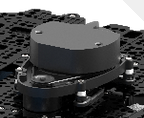
\includegraphics[width=0.1\textwidth]{img/lasersensor.png}\\
	
	Battery: LI-PO 11.1 1800mAh LB-12 19&1&132 &\mylink{https://nodna.de/Robotis-LIPO-111V-Akkupack-1800mAh-LBS-012}{\EUR{44.90}} &
	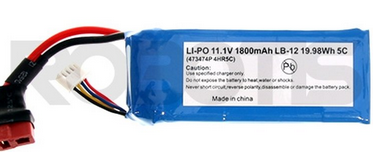
\includegraphics[width=0.1\textwidth]{img/battery.png} \\
	
	Turtlebot3 Layers(125cmx125cm)&4& & & \\
	
	XM430-W350-R Dynamixel (Motors)&3&82 &\mylink{http://support.robotis.com/en/product/actuator/dynamixel_x/xm_series/xm430-w350.htm}{robotis,\EUR{250}} &
	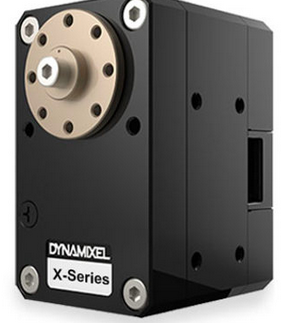
\includegraphics[width=0.1\textwidth]{img/dynamixel.png} \\
	
	Ball(alum., dia.: 140mm, material thickness 2.5mm)&1&400&\mylink{http://www.ball-tech.de/Hohlkugeln/Aluminium/}{ball-tech gmbh,\EUR{40}. } & 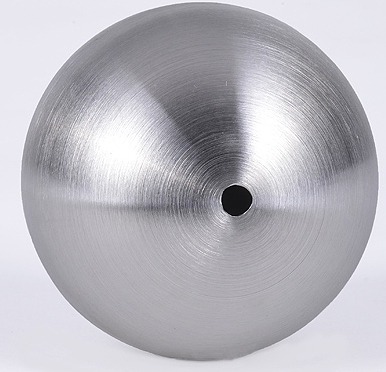
\includegraphics[width=0.1\textwidth]{img/ball.png}\\
	
	Omni wheels(dia: 60mm, thickness:25mm)&3&51.46 &\mylink{http://krause-robotics.de/xtshop/Antriebe/Raeder/Allseitenraeder/Allseitenraeder-60-mm:::99_100_106_114.html}{\EUR{10.38}} &  	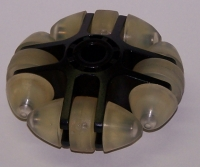
\includegraphics[width=0.1\textwidth]{img/wheel.jpg}   \\
	
	Kreisring (PLA, 3D printeted)&1&28 & & 
	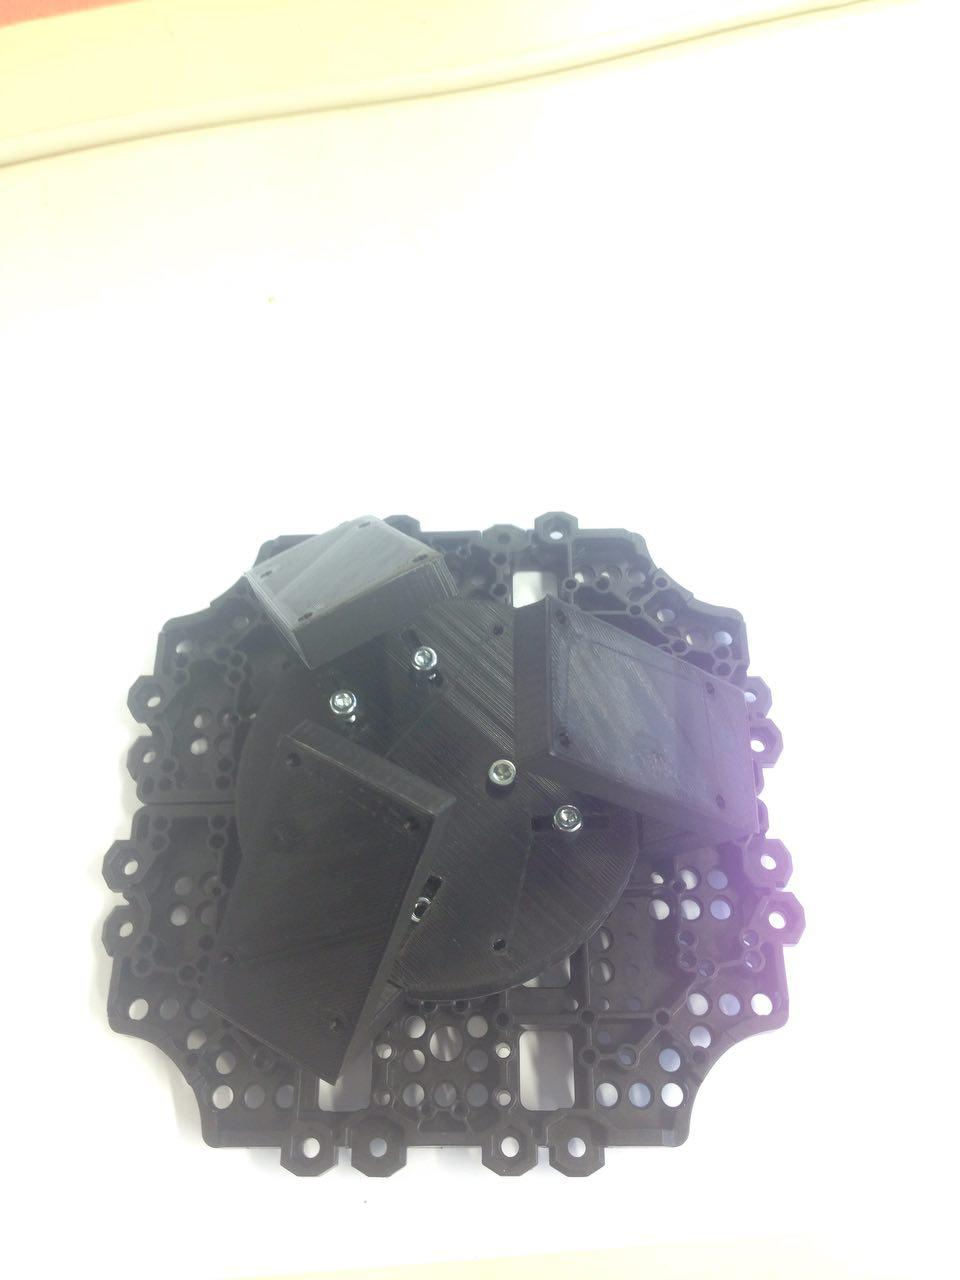
\includegraphics[width=0.1\textwidth]{img/kreisring.png}\\
	
	Halterung (PLA, 3D printeted)&3&18 & & 
	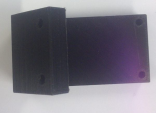
\includegraphics[width=0.1\textwidth]{img/halterung.png} \\
	
	Mitnehmer (PLA, 3D printeted)&3&8 & &
	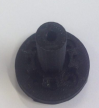
\includegraphics[height=0.06\textwidth]{img/mitnehmer.png}  \\
	
	Plain washer (Beilagscheibe),(PLA, 3D printeted)&3&0.45 & &
	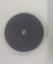
\includegraphics[height=0.06\textwidth]{img/beilagscheibe.png}  \\
	
	M3  (Mutter-Halterung-Kreisring-Layer)&9& & & \\
	M2.5  (Kreisring-Layer)&2& & & \\
	M3x8mm Halterung &6& &Zylinderkopf (Imbus) & \\
	M3x22mm Layer&3&1.34 &Zylinderkopf (Imbus) & \\
	M2.5x22 (Motoren-Halterung) &12&&Sechskant & \\
	M2.5x38 (Motoren-Rad)&3& &Zylinderkopf (Imbus) & \\
	M2.5x24 (Layer)&2& &Zylinderkopf (Imbus) & \\
	M2x6mm  (Mitnehmer-Motor)&12 & &Zylinderkopf (Imbus) & \\
	Distanzbolzen&???& &???& \\
	
\end{tabular}

% Please add the following required packages to your document preamble:
% \usepackage[normalem]{ulem}
% \useunder{\uline}{\ul}{}
\begin{table}[]
\centering
\caption{My caption}
\label{my-label}
\begin{tabular}{|c|c|c|c|}
\hline
{\textbf{Type}} & {\textbf{Size}}                                             & { \textbf{Amount}} & { \textbf{Place}} \\ \hline
Cylinderhead screw  & M3 x 11mm                                                       & 8                     & Motor mounts         \\ \hline
Cylinderhead screw  & M2,5 x 22mm                                                     & 16                    & Motor plate          \\ \hline
Cylinderhead screw  & M2 x 6 mm                                                       & 18                    & Wheel shaft          \\ \hline
Cylinderhead screw  & \begin{tabular}[c]{@{}c@{}}M2,5  x 36 mm\\ (38 mm)\end{tabular} & 5                     & Wheel shaft cover    \\ \hline
Cylinderhead screw  & \begin{tabular}[c]{@{}c@{}}M3 x 20 mm\\ (21mm)\end{tabular}     & 4                     & Layer mounting       \\ \hline
Nut                 & M2                                                              & 5                     & Layer mounting       \\ \hline
Cylinderhead screw  & \begin{tabular}[c]{@{}c@{}}M2,5 x 22mm\\ (23mm)\end{tabular}    & 4                     & Layer mounting       \\ \hline
\end{tabular}
\end{table}


\textbf{Total Cost: \EUR{1176} + Cost of opencr board and all plastic (incl. tb3 structure) and scrwes }

TODO:\\
\begin{enumerate}
	\item Abmessungen von einer struckture layer
	\item upboard1-link noch eintragen
\end{enumerate}

\chapter{Simulation}

TODO: 
check if controller works

check why imu fails

\section{Launch}
These files are executed one after another:
\begin{enumerate}
	\item bb\_simulation: ballbot.launch
	\item bb\_description: bb\_description.launch
	\item bb\_description -> urdf: bb.xacro
	\item bb\_description -> urdf: bb.urdf.xacro
	\item bb\_description -> urdf: common\_properties.xacro
	\item bb\_description -> urdf: bb.gazebo.xacro
\end{enumerate}

\section{Simulation design}

Ballbot SDF Reference:
\mylink{https://bitbucket.org/osrf/gazebo/issues/2335/how-to-set-the-friction-of-ballbot-the}{Ballbotmodel} 

We use not the sdf but the xacro description as in this example \mylink{http://gazebosim.org/tutorials/?tut=ros_urdf}{here}.

\begin{center}
		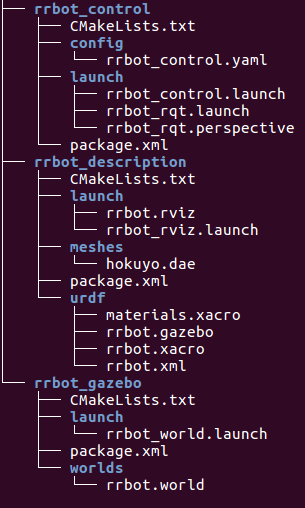
\includegraphics[width=0.2\textwidth]{img/filestructure.png} 
\end{center}

Gazebo uses different physics engines:\\
\begin{itemize}
	\item Open Dynamics Engine (ODE) (Default)
	\item Bullet
	\item Dynamic Animation and Robotics Toolkit (DART)
	\item Simbody
\end{itemize}
 which all have different friction etc. models.

Files:
\begin{itemize}
	\item bb.urdf.xacro: Link's: Visual description of the Robot and its collision model(STL file). Pose Mass and Inertias. Joint's: Pose,axis,effort and velocity limits, friction.
	\item common\_properties.xacro: Macros for color definition.
	\item bb.gazebo.xacro: gazebo references dynamics of the links: friction parameters (mu1,mu2), 
\end{itemize}

Gazebo Parameter's List:\\
\begin{tabular}{l L{12cm} l l}
	name(xacro)&description&value&sdf group\\
	mu1&is the Coulomb friction coefficient for the first friction direction&1.0&ode\\
	mu2& is the friction coefficient for the second friction direction (perpendicular to the first friction direction)&2.0&ode\\
	kp&spring constant equivalents of a contact as a function of SurfaceParams::cfm and SurfaceParams::erp & &ode \\
	kd&spring damping constant equivalents of a contact as a function of SurfaceParams::cfm and SurfaceParams::erp.   & &ode \\
	cfm&Constraint Force Mixing parameter.& &ode \\
	erp&Error Reduction Parameter.& &ode \\
	min\_depth&Minimum depth before ERP takes effect.   & &ode \\
	max\_Vel& Maximum interpenetration error correction velocity.
	If set to 0, two objects interpenetrating each other will not be pushed apart.  & &ode \\
	slip1&Artificial contact slip in the primary friction direction  & &ode \\
	slip2&Artificial contact slip in the secondary friction dirction.& &ode \\
\end{tabular}

See: \mylink{http://osrf-distributions.s3.amazonaws.com/gazebo/api/dev/classgazebo_1_1physics_1_1ODESurfaceParams.html}{ODESurfaceParams}

\section{Gazebo Parameters}

	
	\section{Control}
	sobald diff drive plugin angeschaltet drehen sich die raeder viel zu schnell ....
	
	Diff Drive in ballbot.launch an oder ausschalten. 
	
	in bb.gazebo.xacro transmission und controller festlegen.
	
	zudem yaml file(currently I use: effort\_controllers/JointVelocityController)
	
	Effort Joint Interface as Hardware Interface is used.
	
	Do this example first: \url{http://gazebosim.org/tutorials/?tut=ros_control}
	
	Also try this bb8 gazebo tutorial: \url{https://www.youtube.com/watch?v=j5qC9l448p8}
	
	\subsection{Plugins}
	\begin{itemize}
		\item gazebo-ros-control
		\item diff drive
	\end{itemize}
	
	\subsection{Launch}
	\begin{lstlisting}[style=BashInputStyle]
	roslaunch rrbot_control rrbot_control.launch
	\end{lstlisting}
	
	These files are executed one after another:
	\begin{enumerate}
		\item load config
		\item controller\_spawner
	\end{enumerate}
	
	\section{Sensors}
	\subsection{IMU}
	
		We want to simulate the IMU of the opencr board. STRG+T to see imu topic values!
	\mylink{https://www.youtube.com/watch?v=wXN_7oRHst0}{Imu of opencr board simulated}

	Simulate like this:
	rviz rviz dann als fixed frame nimm: imu\_link. Und add topic imu und waehle als topic ballbot/sensor/imu
	
	The simulated IMU outputs values like: orientation (x,y,z,w), angluar velocity(x,y,z), linear velocity(x,y,z), linear acceleration(x,y,z).
	
	The opencr real IMU gives values like: orientation(x,y,z,w), angular velocity(x,y,z), linear acceleration(x,y,z) see \mylink{OpenCR board IMU }{http://turtlebot3.readthedocs.io/en/latest/appendix\_opencr.html}
	
	\chapter{Model}
	
	\section{Composition}
	The Ballbot consists of three parts, which are depicted in Figure \ref{fig:Structure}.
	
	\begin{itemize}
		\item Body with motors
		\item 3 omni-directional wheels
		\item Ball
	\end{itemize}
	
	
	\begin{figure}[htbp]
		\centering
		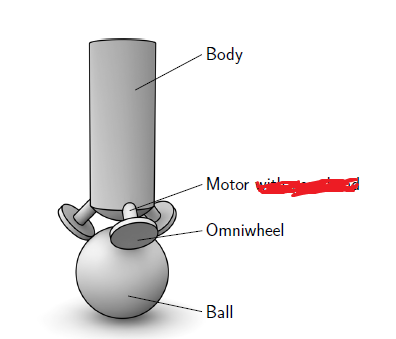
\includegraphics[width=0.9\textwidth]{img/Strucuture.PNG}
		\caption{Parts for the 3D-Model}
		\label{fig:Structure}
	\end{figure}
	
	\section{Assumptions}
	
	To reduce the complexity of the system, the following assumptions are made: 
	
	\begin{itemize}
		\item \textbf{No slip} between the contact points between the ball/ground and wheels/ball
		\item \textbf{No friction}; except the friction, which occurs at the rotation of the ball around the z-axis
		\item \textbf{No deformation}
		\item \textbf{Fast motor dynamics}; The controlling of the motor is much faster than the controller of the Ballbot
		\item \textbf{Ball moves only horizontal}
	\end{itemize}
	
	\section{Model Parameters}
	
	
% Please add the following required packages to your document preamble:
% \usepackage[normalem]{ulem}
% \useunder{\uline}{\ul}{}
\begin{table}[]
\centering
\caption{My caption}
\label{my-label}
\begin{tabular}{cccc}
\hline
\multicolumn{1}{|c|}{{ \textbf{Parameter}}}                                                                          & \multicolumn{1}{c|}{{\textbf{Variable}}} & \multicolumn{1}{c|}{{ \textbf{Value}}}                  & \multicolumn{1}{c|}{{ \textbf{Source}}} \\ \hline
                                                                                                                        &                                              &                                                            &                                            \\ \hline
\multicolumn{1}{|c|}{Mass of the ball}                                                                                  & \multicolumn{1}{c|}{$m_{K}$}                & \multicolumn{1}{c|}{0,4 kg}                                & \multicolumn{1}{c|}{Datasheet}             \\ \hline
\multicolumn{1}{|c|}{Mass of the ball}                                                                                  & \multicolumn{1}{c|}{$m_{K}$}                & \multicolumn{1}{c|}{0,397 kg}                              & \multicolumn{1}{c|}{Measured}              \\ \hline
\multicolumn{1}{|c|}{Mass of the ball}                                                                                  & \multicolumn{1}{c|}{$m_{K}$}                & \multicolumn{1}{c|}{0,631 kg}                              & \multicolumn{1}{c|}{SolidEdge}             \\ \hline
\multicolumn{1}{|c|}{\begin{tabular}[c]{@{}c@{}}Mass of the body, complete\\ (with motors/wheels)\end{tabular}}         & \multicolumn{1}{c|}{$m_{B}$}                & \multicolumn{1}{c|}{?}                                     & \multicolumn{1}{c|}{Measured}              \\ \hline
\multicolumn{1}{|c|}{\begin{tabular}[c]{@{}c@{}}Mass of the body, complete\\ (with motors/wheels)\end{tabular}}         & \multicolumn{1}{c|}{$m_{B}$}                & \multicolumn{1}{c|}{1,785 kg}                              & \multicolumn{1}{c|}{SolidEdge}             \\ \hline
\multicolumn{1}{|c|}{\begin{tabular}[c]{@{}c@{}}Mass of the body\\ (without motors/wheels)\end{tabular}}                & \multicolumn{1}{c|}{$m_{B}$}                & \multicolumn{1}{c|}{?}                                     & \multicolumn{1}{c|}{Measured}              \\ \hline
\multicolumn{1}{|c|}{\begin{tabular}[c]{@{}c@{}}Mass of the body\\ (without motors/wheels)\end{tabular}}                & \multicolumn{1}{c|}{$m_{B}$}                & \multicolumn{1}{c|}{1,394 kg}                              & \multicolumn{1}{c|}{SolidEdge}             \\ \hline
\multicolumn{1}{|c|}{Mass of Omniwheel}                                                                                 & \multicolumn{1}{c|}{$m_{OW}$}               & \multicolumn{1}{c|}{0,050 kg}                              & \multicolumn{1}{c|}{Measured}              \\ \hline
\multicolumn{1}{|c|}{Mass of Omniwheel}                                                                                 & \multicolumn{1}{c|}{$m_{OW}$}               & \multicolumn{1}{c|}{0,046 kg}                              & \multicolumn{1}{c|}{SolidEdge}             \\ \hline
\multicolumn{1}{|c|}{Mass of the virtual wheel}                                                                         & \multicolumn{1}{c|}{$m_{VW}$}               & \multicolumn{1}{c|}{0,384 kg}                              & \multicolumn{1}{c|}{Measured}              \\ \hline
\multicolumn{1}{|c|}{\begin{tabular}[c]{@{}c@{}}Mass of the substructure, complete\\ (with motors/wheels)\end{tabular}} & \multicolumn{1}{c|}{$m_{S}$}                & \multicolumn{1}{c|}{0,506 kg}                              & \multicolumn{1}{c|}{Measured}              \\ \hline
\multicolumn{1}{|c|}{\begin{tabular}[c]{@{}c@{}}Mass of the substructure, complete\\ (with motors/wheels)\end{tabular}} & \multicolumn{1}{c|}{$m_{S}$}                & \multicolumn{1}{c|}{0,457 kg}                              & \multicolumn{1}{c|}{SolidEdge}             \\ \hline
\multicolumn{1}{|c|}{Mass of plate}                                                                                     & \multicolumn{1}{c|}{$m_{P}$}                & \multicolumn{1}{c|}{0,078 kg}                              & \multicolumn{1}{c|}{Measured}              \\ \hline
\multicolumn{1}{|c|}{Mass of plate}                                                                                     & \multicolumn{1}{c|}{$m_{P}$}                & \multicolumn{1}{c|}{?}                                     & \multicolumn{1}{c|}{SolidEdge}             \\ \hline
                                                                                                                        &                                              &                                                            &                                            \\ \hline
\multicolumn{1}{|c|}{Radius of the ball}                                                                                & \multicolumn{1}{c|}{$r_{K}$}                & \multicolumn{1}{c|}{0,07 m}                                & \multicolumn{1}{c|}{Datasheet}             \\ \hline
\multicolumn{1}{|c|}{Radius of the body}                                                                                & \multicolumn{1}{c|}{$r_{B}$}                & \multicolumn{1}{c|}{0,0703 m}                              & \multicolumn{1}{c|}{Measured}              \\ \hline
\multicolumn{1}{|c|}{Radius of the Wheels}                                                                              & \multicolumn{1}{c|}{$r_{W}$}                & \multicolumn{1}{c|}{0,03 m}                                & \multicolumn{1}{c|}{Datasheet}             \\ \hline
\multicolumn{1}{|c|}{Height of the center of gravity}                                                                   & \multicolumn{1}{c|}{$l$}                       & \multicolumn{1}{c|}{0,24045 m}                             & \multicolumn{1}{c|}{SolidEdge}             \\ \hline
\multicolumn{1}{|c|}{Height of the body}                                                                                & \multicolumn{1}{c|}{$h$}                       & \multicolumn{1}{c|}{0,34294 m}                             & \multicolumn{1}{c|}{SolidEdge}             \\ \hline
\multicolumn{1}{|c|}{Inertia of the Ball}                                                                               & \multicolumn{1}{c|}{$\Theta_{K}$}           & \multicolumn{1}{c|}{0,00131 $kgm^{2}$}     & \multicolumn{1}{c|}{Computed}              \\ \hline
\multicolumn{1}{|c|}{Inertia of the Body (x-axis)}                                                                      & \multicolumn{1}{c|}{$\Theta_{Bx}$}          & \multicolumn{1}{c|}{0,08751 $kgm^{2}$}     & \multicolumn{1}{c|}{SolidEdge}             \\ \hline
\multicolumn{1}{|c|}{Inertia of the Body (y-axis)}                                                                      & \multicolumn{1}{c|}{$\Theta_{By}$}          & \multicolumn{1}{c|}{0,08788 $kgm^{2}$}     & \multicolumn{1}{c|}{SolidEdge}             \\ \hline
\multicolumn{1}{|c|}{Inertia of the body (z-axis)}                                                                      & \multicolumn{1}{c|}{$\Theta_{Bz}$}          & \multicolumn{1}{c|}{0,00329 $kgm^{2}$}     & \multicolumn{1}{c|}{SolidEdge}             \\ \hline
\multicolumn{1}{|c|}{Inertia of the body (xy plane)}                                                                    & \multicolumn{1}{c|}{$\Theta_{Bxy}$}         & \multicolumn{1}{c|}{-0,00001 $kgm^{2}$}    & \multicolumn{1}{c|}{SolidEdge}             \\ \hline
\multicolumn{1}{|c|}{Inertia of the body (xz plane)}                                                                    & \multicolumn{1}{c|}{$\Theta_{Bxz}$}         & \multicolumn{1}{c|}{0,00203 $kgm^{2}$}     & \multicolumn{1}{c|}{SolidEdge}             \\ \hline
\multicolumn{1}{|c|}{Inertia of the body(zy plane)}                                                                     & \multicolumn{1}{c|}{$\Theta_{Bzy}$}         & \multicolumn{1}{c|}{0,00018 $kgm^{2}$}     & \multicolumn{1}{c|}{SolidEdge}             \\ \hline
\multicolumn{1}{|c|}{Inertia of the rotor (motor)}                                                                      & \multicolumn{1}{c|}{$\Theta_{M}$}           & \multicolumn{1}{c|}{0,444e-6 $kgm^{2}$}    & \multicolumn{1}{c|}{Adoption}              \\ \hline
\multicolumn{1}{|c|}{Inertia of Omniwheel}                                                                              & \multicolumn{1}{c|}{$\Theta_{OW}$}          & \multicolumn{1}{c|}{0.000023157 $kgm^{2}$} & \multicolumn{1}{c|}{Computed}              \\ \hline
\multicolumn{1}{|c|}{Inertia of the actuating wheel in yz/xz}                                                            & \multicolumn{1}{c|}{$\Theta_{W}$}           & \multicolumn{1}{c|}{0,058873 $kgm^{2}$}    & \multicolumn{1}{c|}{Computed}              \\ \hline
\multicolumn{1}{|c|}{Inertia of the actuating wheel in xy}                                                              & \multicolumn{1}{c|}{$\Theta_{Wxy}$}         & \multicolumn{1}{c|}{0,16656 $kgm^{2}$}     & \multicolumn{1}{c|}{Computed}              \\ \hline
                                                                                                                        &                                              &                                                            &                                            \\ \hline
\multicolumn{1}{|c|}{Gear ratio}                                                                                        & \multicolumn{1}{c|}{$i$}                       & \multicolumn{1}{c|}{353,5}                                 & \multicolumn{1}{c|}{Datasheet}             \\ \hline
\multicolumn{1}{|c|}{Gravitational acceleration}                                                                        & \multicolumn{1}{c|}{$g$}                       & \multicolumn{1}{c|}{9,81 $m/s^{2}$}        & \multicolumn{1}{c|}{BachelorThesis}        \\ \hline
\end{tabular}
\end{table}

Traegheitsmoment kugel Hohlzylinder: $J=m \frac{r_i^2+r_a^2}{2} = 0.4 * \frac{65^2+70^2}{2} kg *10^ {-6} m^2=1.825 *10^{-3} kg m^2$ 

Traegheitsmoment wheel Vollzylinder: $J=m \frac{1}{2} r^2 = 0.05146 * 0.020^2 = 1.0292 * 10^{-4} kg m^2$ 
	
	
\end{document}
